\section*{III.1.1}
\subsection*{Verification of gradient computations}
Please see \texttt{III\_1\_1.m} which calculates the
numerically estimated gradients and verifies that the
difference between those and the weights calculated by
one round of forward/backward propagation is very small.

\subsection*{Derivative of $h(a)$}
In the following we asume $a\neq0$.

\begin{align*}
  h(a) &= \frac{a}{1 + |a|} \\
  \left(\frac{f}{g}\right)' &= \frac{f'g - g'f}{g^2} \\
  f(a) &= a \\
  f'(a) &= 1 \\
  g(a) &= 1 + |a| \\
  g^2(a) &= (1 + |a|)^2 \\
  g'(a) &= \frac{|a|}{a} \\
  h'(a) &= \frac{1(1 + |a|) - \frac{|a|}{a}a}{(1 + |a|)^2} \\
        &= \frac{1 + |a| - |a|}{(1 + |a|)^2} \\
        &= \frac{1}{(1 + |a|)^2}
\end{align*}

\section*{III.1.2}
\subsection*{What happens for small/large learning rates?}
The smaller the learning rate, the less you adjust weights by and thus the smaller
steps you take during each epoch of gradient descent. Conversely, the larger the learning rate, 
the bigger a factor weights are adjusted by and the bigger steps you take during each epoch of
gradient descent.

Beyond concerns about running time, a small learning rate may risk getting stuck in a very small
local minimum and bigger learning rates risk bounding off past a good minimum. Selecting a good
learning rate can thus be a case of trial and error, such as starting with a large learning rate
to sketch out the general topology of the gradient and then switching to lower learning rates
afterwards.

\begin{figure}[h!]
  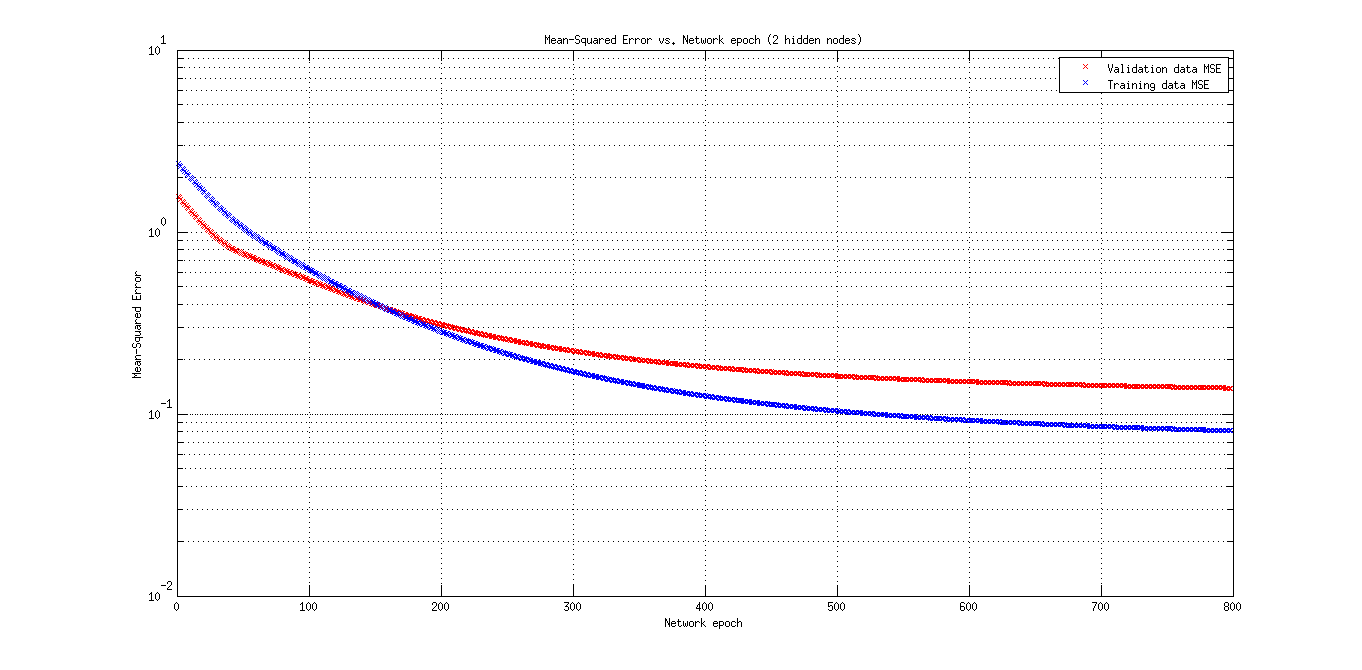
\includegraphics[width=\linewidth]{images/mse2.png}
  \caption{Mean-Squared-Error across epochs, for a Neural Network with 2 hidden nodes.
  \label{fig:mse2}}
\end{figure}

\begin{figure}[h!]
  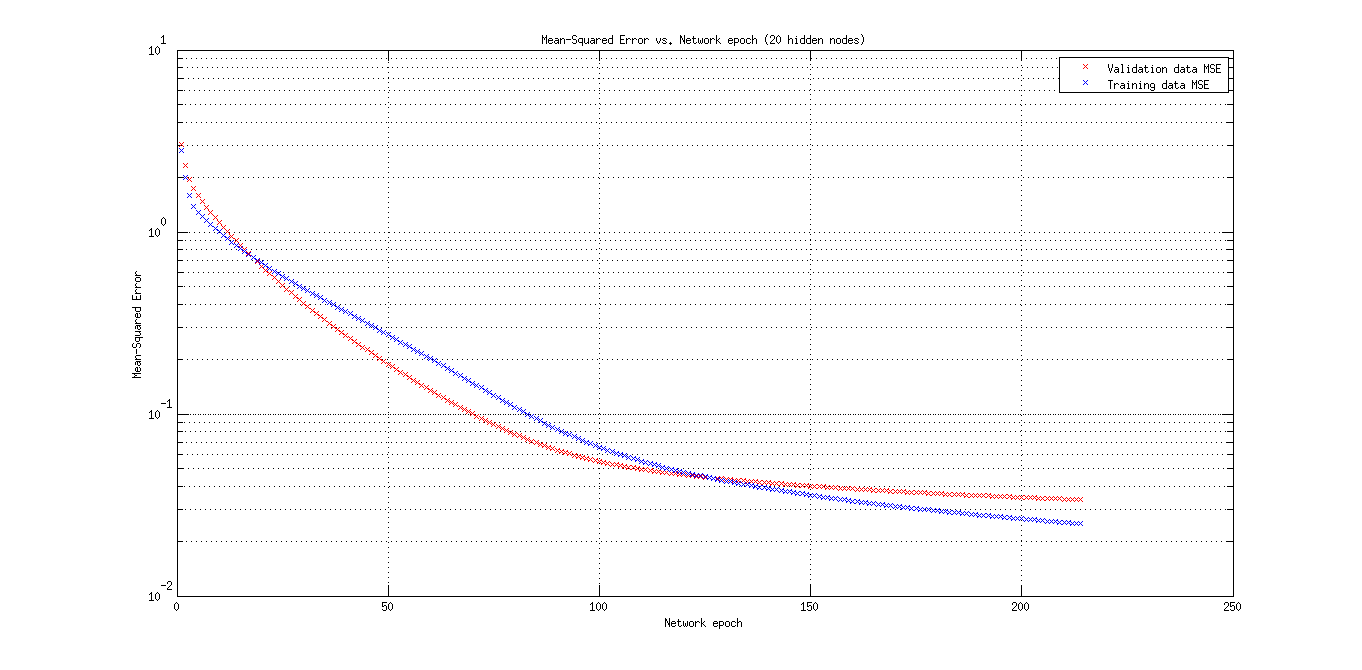
\includegraphics[width=\linewidth]{images/mse20.png}
  \caption{Mean-Squared-Error across epochs, for a Neural Network with 20 hidden nodes.
  \label{fig:mse20}}
\end{figure}

Figure~\ref{fig:mse2} and Figure~\ref{fig:mse20} show the Mean-Squared Error (MSE) of the two
neural networks across learning epochs. In both cases we see a steady decrease in error, however
the error of the 20-node network is significantly lower than the 2-node network. It is probable that
our 2-node network is incapable of illustrating the kind of distribution that the data stems from,
causing severe issues for certain data points.

\subsection*{Sinc vs. Neural Network}
Figures~\ref{fig:sinc2} and~\ref{fig:sinc20} show the \texttt{sinc(x)} function across the range
$[-10; 10]$ alongside neural networks with 2 and 20 nodes respectively. The network with 2 nodes
fits the data roughly like two functions of the kind $f(x)=a/(1+norm(a))$ strung together with linear
weight coefficients. Increasing the number of nodes to 20 allows the linear combination of weights
and inputs and activations to express a distribution closer to that of \texttt{sinc(x)}.

\begin{figure}[h!]
  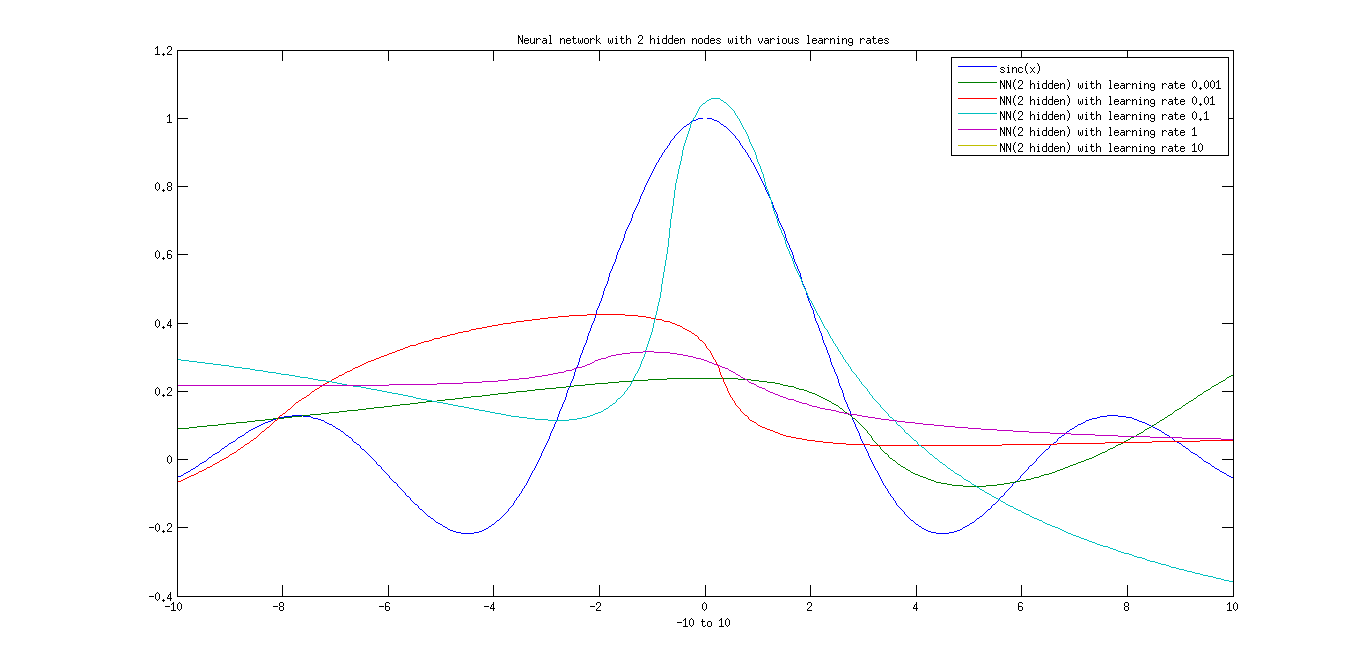
\includegraphics[width=\linewidth]{images/sinc2.png}
  \caption{sinc(x) vs. Neural Network with 2 hidden nodes, plotted across the range [-10; 10]
  \label{fig:sinc2}}
\end{figure}

\begin{figure}[h!]
  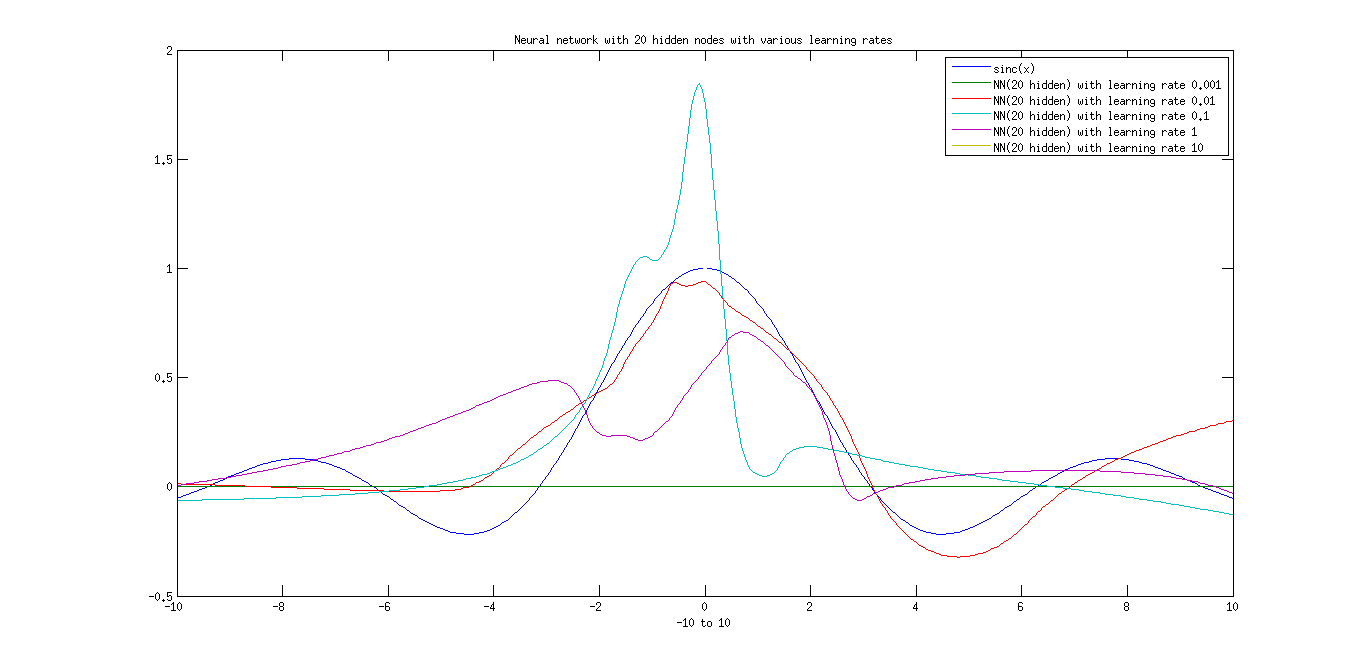
\includegraphics[width=\linewidth]{images/sinc20.png}
  \caption{sinc(x) vs. Neural Network with 20 hidden nodes, plotted across the range [-10; 10]
  \label{fig:sinc20}}
\end{figure}

\subsection*{Overfitting and early stopping}
Overfitting occurs when a fit becomes overly complex and tied to the data being used to train with.
One solution to overfitting is to include a regularization parameter in order to lessen the effects
of overfitting. Another solution is to perform early stopping: when training an optimization algorithm,
the error measured with respect to independent data (such as a validation set) often shows a decrease
at first, followed by an increase. We can stop at the point where the error on the validation set
increases, in order to obtain a network that hopefully has better generalization performance than had
we continued.

\section*{III.2.1}
\textbf{Mean/variance of the training data}\\
\begin{tabular}{|r|r|r|r|r|r|}
\hline
priorTrainMean & priorTrainVar & trainMean & trainVar & testMean & testVar \\\hline
         &$1.0e+03 *$ & $1.0e-14 *$ & & & \\
155.9604 & 1.9830 &  0.0180 & 1.0000 & -0.0782 & 0.7323 \\
204.8212 & 9.7331 & -0.0623 & 1.0000 & -0.1572 & 0.7150 \\
115.0586 & 2.1152 & -0.0305 & 1.0000 &  0.0553 & 0.7977 \\
  0.0060 & 0.0000 &  0.0151 & 1.0000 &  0.1126 & 1.9906 \\
  0.0000 & 0.0000 & -0.1268 & 1.0000 &  0.0712 & 1.6662 \\
  0.0032 & 0.0000 & -0.0344 & 1.0000 &  0.0865 & 2.1370 \\
  0.0033 & 0.0000 &  0.0238 & 1.0000 &  0.1151 & 1.9225 \\
  0.0096 & 0.0000 & -0.0019 & 1.0000 &  0.0866 & 2.1379 \\
  0.0277 & 0.0000 &  0.1217 & 1.0000 &  0.2477 & 1.7721 \\
  0.2624 & 0.0000 & -0.0762 & 1.0000 &  0.2439 & 1.8292 \\
  0.0147 & 0.0000 &  0.1304 & 1.0000 &  0.2284 & 1.7175 \\
  0.0166 & 0.0000 & -0.0491 & 1.0000 &  0.2496 & 1.7780 \\
  0.0220 & 0.0000 &  0.0597 & 1.0000 &  0.3150 & 2.1905 \\
  0.0440 & 0.0000 & -0.0129 & 1.0000 &  0.2284 & 1.7176 \\
  0.0226 & 0.0000 &  0.0140 & 1.0000 &  0.1483 & 2.6633 \\
 22.0007 & 0.0167 & -0.2299 & 1.0000 & -0.0565 & 1.3610 \\
  0.4948 & 0.0000 &  0.1184 & 1.0000 &  0.0732 & 1.0827 \\
  0.7157 & 0.0000 &  0.3141 & 1.0000 &  0.0863 & 0.9514 \\
 -5.7637 & 0.0011 & -0.1559 & 1.0000 &  0.1540 & 1.2166 \\
  0.2148 & 0.0000 &  0.0715 & 1.0000 &  0.3091 & 1.3629 \\
  2.3658 & 0.0001 & -0.1414 & 1.0000 &  0.0870 & 1.1336 \\
  0.1997 & 0.0000 & -0.0476 & 1.0000 &  0.1677 & 1.4149 \\\hline
\end{tabular}

\section*{III.2.2}

\textit{Description of the software used:}\\
We used LibSVM for
Matlab\footnote{\url{http://www.csie.ntu.edu.tw/\~cjlin/libsvm/\#matlab}}.
Training the SVM produces a model structure, this is done like so:
\begin{verbatim}
model = svmtrain(trainX, trainY, 'kernel_function','rbf',
                 'rbf_sigma',sigmas,'boxconstraint',C);
\end{verbatim}


\begin{tabular}{|l l|}
\hline
trainX                      & Training data features.\\
trainY                      & Corresponding training data classes.\\
'kernel\_function' \& 'rbf' & Sets the kernel function to be a gaussian kernel function.\\
'rbf\_sigma' \& sigmas      & Lets us specify a $\sigma = \sqrt{1/(2\gamma)}$.\\
'boxconstraint' \& C        & Lets us specify regularization paramter.\\\hline
\end{tabular}

\noindent \textit{Our process:}\\
For our five-fold cross validation we re-used the code (\texttt{shuffleSplit}
and \texttt{bucketJoiner}) from the first assignment. So for each C and each
$\gamma$ we did a five-fold cross validation. The best C and Gamma combination
was extracted and used to train a new model that could be used for
classification.

\noindent \textit{Results:}\\
We used the following numbers for $C$ and $\gamma$: $C = (0.01, 0.1, 1.0, 10,
100, 1000, 10000)$ and $\gamma = (0.0001, 0.001, 0.01, 0.1, 1, 10, 100)$. For
the raw data we found the best $C$ and $\gamma$ to be $C=0.01,
\gamma=0.001$. For the normalized data we found $C=100, \gamma=0.1$.

\begin{tabular}{l l}
Prenormalized training data accuracy & $ 46.94\%$\\
Prenormalized test data accuracy     & $ 46.39\%$\\
Normalized training data accuracy    & $100.00\%$\\
Normalized test data accuracy        & $ 89.69\%$\\
\end{tabular}

\noindent \textit{Discussion:}\\
If you do not normalize your data, you will unwillingly give more importance to
feutures wich are widely spreed, and similarly give less importeanse to dense
data.

\section*{III.2.3.1}
For our optimum hyper-parameters the number of free support vectors are $0$, and
the number of bound support vectors are $54$. Changing $C$ will change the
number of support vectors in the model, a lower value of $C$ will result in more
support vectors and with more free support vectors. This means smaller $C$
values gives you more support vectors to work with, but the increase in free
support vectors also means that the machine is more prone to
miss-classification.

\section*{III.2.3.2}
As the number of entries in the training data increases so does the number of
support vectors in the SVM. The amount of free vectors (for our training
dataset) is roughly one third of the total number of support vectors and the
ratio seems to converge as the total number of support vectors increase. The
increase in the number of support vectors will mean the SVM takes more time to
process each query afterwards, but will also be able to do so with greater
accuracy. So much like the $C$ value, this becomes a trade-off, in this case
between accuracy and speed.
